\documentclass{report}
\usepackage[T1]{fontenc} % Fontes T1
\usepackage[utf8]{inputenc} % Input UTF8
\usepackage[backend=biber, style=ieee]{biblatex} % para usar bibliografia
\usepackage{csquotes}
\usepackage[portuguese]{babel} % Usar língua portuguesa
\usepackage{blindtext} % Gerar texto automaticamente
\usepackage[printonlyused]{acronym}
\usepackage{hyperref} % para autoref
\usepackage{graphicx}
\usepackage[normalem]{ulem}
\useunder{\uline}{\ul}{}
\usepackage[table,xcdraw]{xcolor} % Para o uso de tabelas coloridas
\usepackage{floatrow} %Imagens lado a lado
\bibliography{bibliografia}

\begin{document}
%% Caminhos das imagens %%
%

%
%% Definições %%
%
\def\titulo{Fórmula 1}                                 
\def\data{25 de novembro de 2019}
\def\autores{André Clérigo, João Castanheira}
\def\autorescontactos{(98485) andreclerigo@ua.pt, (97512) joaocastanheira@ua.pt}
\def\versao{Primeira versão}
\def\departamento{Departamento de Eletrónica, Telecomunicações e Informática}
\def\empresa{Universidade de Aveiro}
\def\logotipo{Fotos/ua.pdf}
%
%%%%%% CAPA %%%%%%
%
\begin{titlepage}

\begin{center}
%
\vspace*{50mm}
%
{\Huge \titulo}\\ 
%
\vspace{10mm}
%
{\Large \empresa}\\
%
\vspace{10mm}
%
{\LARGE \autores}\\ 
%
\vspace{30mm}
%
\begin{figure}[h]
\center
\includegraphics{\logotipo}
\end{figure}
%
\vspace{30mm}
\end{center}
%
\begin{flushright}
\versao
\end{flushright}
\end{titlepage}

%%  Página de Título %%
\title{%
{\Huge\textbf{\titulo}}\\
{\Large \departamento\\ \empresa}
}
%
\author{%
    \autores \\
    \autorescontactos
}
%
\date{\data}
%
\maketitle

\pagenumbering{roman}
%%%%%% Resumo %%%%%%
\renewcommand{\abstractname}{Resumo}
\begin{abstract}

O primeiro objetivo deste relatório é dar a conhecer à comunidade o grande mundo da \ac{f1}, bem como explicar a sua historia e a maneira em que o desporto se encontra. Visa também referir e dar a conhecer tudo o que envolve um \ac{gp} e a maneira como se processa, além de dar a conhecer as equipas que participam atualmente na categoria e os pilotos que as representam. Além disso, são também referidas todas as regras, penalizações e bandeiras usadas para conseguir estabelecer uma comunicação com os pilotos em pista. Por fim, são enunciadas os impactos que a \ac{f1} tem no nosso quotidiano, assim como são dadas a conhecer algumas curiosidades.

Este projeto foi criado no code.ua.pt com o nome labi2019-t3g02.
\end{abstract}

%%%%%%%%%%%%%%%%%%%%%%%%%%%%
%%%%%% Agradecimentos %%%%%%
\renewcommand{\abstractname}{Agradecimentos}
\begin{abstract}

Para a realização deste primeiro trabalho de aprofundamento para a disciplina de  \ac{labi}, temos que agradecer ao professor Óscar Narciso Mortágua Pereira pelos ensinamentos relativamente à utilização do {\LaTeX}. Agradecemos também o apoio prestado pelos nossos colegas de curso e principalmente ao João Trindade, ao Tomás Freitas e à Luísa Amaral pelos diversos esclarecimentos de dúvidas e pelo fornecimento de opinião quando requerida.
\end{abstract}

%%%%% Conteúdos %%%%%
\tableofcontents
\listoftables     
\listoffigures   

%%%%%%%%%%%%%%%%%%%%%%%%%%%%%%%
\clearpage
\pagenumbering{arabic}

%%%%%%%%%%%%%%%%%%%%%%%%%%%%%%%%
\chapter{Introdução}
\label{chap.introducao}
\hspace{\parindent}Este é um trabalho de aprofundamento para a disciplina de \ac{labi} no curso de \ac{miect} tem como tema a prova rainha dos desportos motorizados, a \ac{f1}.
Este documento está dividido em 7 capítulos. \cite{enciclopediaf1}

Depois desta introdução, no \autoref{chap.histf1} é apresentada a história deste desporto, a maneira como evoluiu, assim como equipas que foram importantes para a evolução do desporto.

No \autoref{chap.f1atual} é nos apresentado as equipas que competem atualmente, assim como os seus pilotos e os monolugares de cada equipa. É nos também explicado a maneira como se processa um Grande Prémio, assim como as pistas atuais no calendário da \ac{f1}, referindo também a evolução de marketing que o desporto sofreu.

O \autoref{chap.regras} refere todas as regras, bandeiras usadas e penalizações que advêm do não cumprimento destas.

No \autoref{chap.impactof1} são apresentadas as inovações que foram primeiramente usadas na \ac{f1} e que depois foram transportadas para o nosso quotidiano, sendo seguido pelo \autoref{chap.curiosidades} que nos presenteia com algumas curiosidades interessantes do desporto.

Por fim, no \autoref{chap.conclusoes}, referimos as conclusões e o que aprendemos com a realização deste trabalho.

\chapter{História da Fórmula 1}
\label{chap.histf1}

\section{\ac{f1} no passado}
\hspace{\parindent}O campeonato de \ac{f1} conta com 60 anos de história, sendo que este passou por várias fases e várias etapas. A primeira época distinta deste campeonato que decorreu desde 1950 a 1958, contou com o retorno da competição automobilística depois desta ter sido interrompida por causa da Segunda Guerra Mundial. Este período contou com o domínio de equipas que já tinham participado em competições antes da pausa devido à guerra. Assim, viu-se o domínio de equipas como a Alfa Romeo, Ferrari, Mercedes-Benz e Maserati. Nestas primeiras temporadas foram usados carros que já tinham sido usados antes da guerra. Estes carros tinham motor dianteiro, pneus estreitos e um motor de 1,5 \ac{cc} com condensador ou 4,5\ac{cc} sem condensador. Até 1954 existiu apenas um campeonato na prova, sendo este o dos pilotos. Depois dessa data, passou a existir também um campeonato de equipas construtoras.\vspace{5mm}

De 1959 a 1980, existiu a denominada época dos garagistas, em que a aerodinâmica foi ganhando importância, A pressão da força aerodinâmica era tão grande que se tornou imperativo desenvolver molas extremamente duras para manter a altura do carro constante e assim conseguir obter uma suspensão mais competitiva. Esta época ficou conhecida por época dos garagistas, uma vez que os carros eram desenvolvidos e aprimorados nas garagens das equipas, em vez de nas fábricas.\vspace{5mm}

A partir dos anos 80 e até ao início do século XXI, a \ac{f1} começou a ser o grande negócio que nos é apresentada hoje em dia. Pelas mãos de Bernie Ecclestone, que desde 1970 geria os direitos comerciais da \ac{f1}, esta foi-se transformando num negócio de milhões de euros. Após a compra da equipa Brabham, em 1971, Bernie conseguiu obter um lugar na \ac{foca} e em 1978 tornou-se presidente desta mesma associação.
A monopolização do poder e o controlo que Bernie Ecclestone tinha na \ac{f1}, levou Jean Marie Ballestre a criar a \ac{fisa}, que veio travar uma guerra de dez anos contra a \ac{foca} pela exploração da \ac{f1}. Esta guerra só terminou quando Enzo Ferrari interveio e as duas entidades assinara o Acordo de Concórdia, que entregou os direitos comerciais à \ac{foca} e a responsabilidade pelos regulamentos técnicos e desportivos da \ac{f1} à \ac{fisa}.\vspace{5mm}

De 2000 a 2007, as regras foram alteradas constantemente, sempre com o objetivo de ter corridas mais emocionantes, reduzir os custos e evitar a manipulação dos resultados. Depois de um longo período, iniciado nos meados dos anos 80, em que a \ac{f1} tinha como os seus principais competidores as equipais especializadas em corridas, como  a Williams, McLaren e Benetton, usando motores fornecidos pelas grandes fábricas, a \ac{f1} voltou a ser dominada pelas equipas produtoras de motores. Começou com a criação, pela Ford, da Jaguar, e levou a um domínio destes fabricantes a partir de 2006, com  o retorno da Renault à competição, a presença da BMW, Toyota, Honda e da Ferrari, e mesmo da McLaren, que não sendo uma equipa produtora de motores, passou a ter uma participação importante da Mercedes-Benz.\vspace{5mm}

Após 2008 as equipas privadas passaram a ser a maioria na categoria, uma vez que se procedeu o abandono de equipas fabricantes. A primeira a deixar a categoria foi a Honda, que oficializou a sua saída no fim de 2008, com promessa de voltar em 2015, como assim aconteceu. Nos ano a seguir, a categoria ficou marcada pela desistência da Toyota e da Renault.\footnote[1]{ps://www.motorsport.com/f1/news/five-of-the-best-f1-innovations-found-through-loopholes/3222390/ (consultado a 26 de novembro de 2019)}

\section{Equipas que mais contribuíram para o desporto}

\hspace{\parindent}Desde cedo que as equipas tiveram um forte peso nas regras da categoria, quer fosse pela procura de falhas no regulamento que permitiram ganhar vantagens sobre os concorrentes, quer fosse pelo desenvolvimento tecnológico, que tornou a categoria como o pináculo em termos de tecnologia automóvel. Assim, algumas equipas que se destacaram ao longo dos tempos foram:
\begin{itemize}
  \item \textbf{Alfa Romeo -} com o \textit{Alfa Romeo 158}, que praticamente decidiu o formato dos carros, e que se mantém até agora. Com o carro a pesar pouco mais de 600kg e a produzir mais de 600\ac{bhp}, este carro levou Giuseppe Farina ao seu primeiro campeonato em 1950 e o seu sucessor, o \textit{Alfa Romeo 159} levou-o ao título em 1951.
  \item \textbf{Cooper -} com o \textit{Cooper T51 Climax}, foi usado pela primeira vez o motor atrás do piloto, o que permitiu aos carros terem um nariz mais aerodinâmico, e um centro de gravidade mais baixo. Com estas alterações, a Cooper ganhou o campeonato de 1959 e 1960, tendo as outras equipa efectuado estas alterações no seu carro em 1961.
   \item \textbf {Renault -} a Renault entrou no desporto em 1977, anunciando o primeiro carro de \ac{f1} que tinha um motor turbo. Apesar de algumas queixas por parte dos pilotos devido ao turbo, a Renault conseguiu ser um forte competidora, conseguindo obter posições de pódio constantemente. A partir de 1983 todos os carros passariam a usar motores turbo. A Renault foi a equipa que em 2006 desenvolveu um sistema para ajudar com as vibrações do carro, e assim garantir dois campeonatos seguidos. Este sistema tinha basicamente o carro apoiado em duas molas, o que foi depois considerado ilegal e banido da competição em 2006.
   \item \textbf{McLaren -} a McLaren foi a primeira equipa a sentar o piloto no carro da maneira como nos é apresentada hoje. Com o \textit{McLaren MP4/4}, um dos carros mais dominantes de sempre, que apresentava um perfil aerodinâmico muito baixo, aliado ao material do chassis desenvolvido pela McLaren, a equipa encontrou o sucesso e garantiu múltiplos campeonatos do mundo, sendo uma das equipas mais bem sucedidas de sempre.
    \item \textbf{Williams -} Com o \textit{Williams FW14B}, foi apresentado pela primeira vez ao mundo o primeiro sistema de tração mais proficiente e que dava uma vantagem enorme sobre as outras equipas.A combinação de uma suspensão ativa pré-programada aliada ao controlo de tração ajudou Nigel Mansell, campeão de 1992 a ganhar o título desse ano, depois de ganhar as primeiro cinco corridas.
    \item \textbf{Ferrari - } Desde o início da \ac{f1} que a Ferrari se encontra na competição, sendo sempre uma equipa que obteve resultados invejáveis e foi sempre importante no desenvolvimento da categoria e dos carros. É a única equipa com poder de veto nos regulamentos, o que mostra o peso que esta marca tem na competição. \footnote[2]{http://edition.cnn.com/2014/03/12/sport/motorsport/10-cars-that-changed-formula-one/index.html (consultado a 26 de novembro de 2019)}
\end{itemize}
\chapter{Fórmula 1 Atual}
\label{chap.f1atual}
\begin{figure}[h]
\centering

\includegraphics[scale=0.1]{Fotos/logo_f1.png}
\caption{Logótipo atual da \ac{f1}.}
\label{logof1}
\end{figure}
\hspace{\parindent}A \ac{f1} atual conta com um misto de equipas produtoras de motores e com equipas clientes. Apesar de, em épocas anteriores, existir um domínio das equipas fabricantes, o mesmo não se verifica nesta nova época, como é possível ver pela forte competitividade de equipas como a Aston Martin Red Bull Racing, a McLaren Renault F1 e a Alfa Romeo Ferrari. Apesar de não haver vantagens para as equipas produtoras, desde 2014 que o campeonato tem sido completamente dominado pela Mercedes-Benz, a equipa alemã que conta com o hexacampeão mundial Lewis Hamilton, para os liderar e manter o seu domínio na categoria.
\section{Características de um \ac{gp}}
\hspace{\parindent}Um \ac{gp} é uma prova que decorre desde quinta-feira a domingo e que é constituída por cinco sessões, sendo que três destas são sessões de treino, e as restantes são as sessões de qualificação e a de corrida.
Na quinta-feira são apenas realizadas entrevistas aos pilotos e aos diretores de equipa, assim como alguns espetáculos no recinto da corrida. Na sexta-feira, começa a ação e todo o trabalho que as equipas necessitam para ter uma corrida proveitosa. Neste dia decorrem dois treinos-livres,às 10h00 locais e outro às 14h00 locais, em que as equipas vão testando várias configurações e vários tipos de pneus, de maneira a saberem reagir à pista e às alterações climáticas que podem ocorrer durante a hora da corrida. Durante o sábado, decorre mais um treino-livre, sendo este às 11h00 locais. Os treinos têm durações diferentes, sendo que o primeiro e o segundo duram 1h30 minutos e o último treino dura apenas uma hora.

Às 14h00 de sábado começa a sessão que terá um enorme impacto na corrida, a sessão de qualificação. Esta sessão é composta por três partes, a qualificação 1 (Q1) em que os 5 pilotos que fizeram a volta mais lenta são impedidos de participar na qualificação 2 (Q2) e vão ocupar os últimos cinco lugares das posições de partida. Na Q2 usa-se o mesmo princípio e os 5 pilotos com as voltas mais lentas irão ocupar os lugares desde a 10ª à 15ª posição. Esta parte da qualificação é muito importante, pois os pilotos que avançam para a qualificação 3 (Q3), ou seja os 10 mais rápidos, terão de começar a corrida com os pneus com que fizeram a volta mais rápida na Q2. A Q3 conta com os 10 pilotos que apresentaram os tempos mais rápidos nas sessões de qualificação anteriores e é a mais competitiva, uma vez que se vai decidir quem sairá da primeira posição (pole position) e quem estará em posições competitivas o suficientes para desafiar e incomodar quem vai sair do primeiro lugar.

No domingo, às 14h10 locais, a corrida começa e os pilotos têm de efetuar o número de voltas suficientes para fazer 305km. Caso a corrida exceda os 120 minutos, esta será terminada e os lugares serão atribuídos conforme estavam aquando do fim da corrida.

As horas de início das sessões mudam em certos \ac{gp} devido a, maioritariamente, tradições. Um exemplo disso é o \ac{gp} de Singapura, em que a corrida decorre durante a noite, para, no final da corrida, ser possível ver os tradicionais fogos de artifício característicos da cidade. 

Além disto, existem outros elementos adjuntos a um \ac{gp} que devem ser mencionados. O \ac{sc}, é um veículo que é accionado no momento em que acontece algum sinistro que torna a pista impossível de se circular. O \ac{sc} irá impôr a velocidade máxima a que todos os pilotos atrás dele podem andar, sendo que a ultrapassagem de outro piloto ou do \ac{sc} enquanto este está ativo acabará em penalização. Este voltará para as boxes, quando os comissários considerarem que a pista está novamente segura para circular, dando assim reinício à corrida.

Outro evento muito característico é a cerimónia do pódio, em que os três pilotos que acabarem a corrida em menos tempo, irão ser condecorados, recebendo um troféu alusivo ao \ac{gp}. A equipa que terminar em primeiro lugar receberá também um prémio de equipa.
\section{Equipas atuais}

As 10 equipas que participam na última temporada de \ac{f1} são: \cite{formula1}
\begin{itemize}
    \item \textbf{Alfa Romeo Racing -}  uma das primeiras equipas a competir nesta categoria, tendo estado afastada do desporto durante muitos anos, voltou agora como uma equipa de meio da tabela que está a conseguir obter muito bons resultados, tendo como equipa fornecedora de motores a Ferrari. O seu diretor de equipa é Frederic Vasseur.
    \item \textbf{Scuderia Ferrari -}  a lendária equipa italiana que nunca abandonou o desporto, vem a recuperar de uma má fase e de um jejum de títulos que já vem desde 2007, quando ganhou o seu último mundial de pilotos com um jovem Kimi Räikkönen. Produz os seus próprios motores e conta com Matia Binnoto como diretor de equipa.
    \item \textbf{Red Bull Toro Rosso Honda –} a equipa secundária da Aston Martin Red Bull Racing apresenta-se como uma equipa de captação e de filtração de pilotos para depois ascenderem para a equipa principal. Assim sendo, são uma equipa competitiva de meio da tabela, que por vezes consegue surpreender, como por exemplo aquando da \textbf{vitória} de Sebastian Vettel no \textbf{\ac{gp} de Monza}.
    \item \textbf{Mercedes-AMG Petronas Motorsport -} esta equipa, que voltou ao desporto em 2010, depois de uma pausa de quase 60 anos, tem sido a equipa mais dominante desta fase da \ac{f1}, contando com todos os títulos, quer de equipa, quer de pilotos desde 2014. Esta equipa é conhecida pela sua maestria em executar estratégias diferentes de todas as outras equipas e conseguir obter ótimos resultados com isso. Conta com Toto Wolff como diretor de equipa.
    \item \textbf{ROKiT Williams Racing –} outrora a equipa mais dominante da competição, a Williams passa agora por uma fase negra da sua história. Não tendo conseguido adaptar-se ao regulamento, desde 2017 que esta equipa tem produzido carros muito pouco competitivos e que usualmente acabam as corridas nas últimas posições. Apesar de usar motor Mercedes, o carro tem-se apresentado muito fraco aerodinamicamente, sendo impossível acompanhar o resto das equipas em prova. Conta com a filha do fundador, Claire Williams, para voltar a tentar trazer a glória de volta a esta equipa.
    \item \textbf{Aston Martin Red Bull Racing -} depois de um período de ouro com Sebastian Vettel e Mark Webber tendo como responsável pela criação dos carros Adrian Newey, esta equipa luta pelos campeonatos a par da Ferrari, sendo a terceira equipa mais competitiva, neste momento. Assinou este ano um contrato com a Honda, para o fornecimento dos motores, depois de terminar uma relação outrora super produtiva com a Renault. Tem como diretor de equipa o mediático Christian Horner.
    \item \textbf{Haas \ac{f1} Team -} sendo a equipa mais recente de todas, e sendo a única equipa americana, a Haas teve em 2017 e 2018 umas épocas de sonho, lutando pelo quarto lugar no Mundial de Construtores contra a experiente Renault, apesar de os primeiros estarem na sua época de estreia. Usa motores Ferrari e tem como diretor de equipa Guenther Steiner.
    \item \textbf{McLaren \ac{f1} Team -} contando sempre com pilotos do mais alto calibre (Ayrton Senna, Lewis Hamilton, Alain Prost, Mika Häkkinen), é, a par da Ferrari uma das equipas com mais história e mais títulos. Tendo o seu último título em 2008 com  Lewis Hamilton, esta equipa está num caminho de retorno à glória. A aposta no motor Renault parece ter sido acertada para esta equipa, uma vez que na temporada corrente, a McLaren conseguiu fazer a sua melhor temporada desde 2014. Apesar deste sucesso, assinou um contrato de fornecimento de motores com a Mercedes para 2021. Zak Brown é o diretor da equipa.
    \item \textbf{Sport Pesa Racing Point \ac{f1} Team -} uma equipa renascida das cinzas, a Racing Point foi o resultado depois do colapso da outrora competitiva Force India devido a esquemas ilícitos pelo dono da equipa. Esta equipa é uma equipa que costuma terminar no top 10, tendo como fornecedor de motor a Mercedes. É a equipa mais constante no pódio, a seguir à Mercedes, Ferrari e Red Bull. É uma equipa que conta com um departamento de engenharia muito bom, que consegue fazer o melhor mesmo com poucos recursos. Esta equipa conta com Andy Stevenson como o seu diretor de equipa.
    \item \textbf{Renault F1 Team -} esta equipa é a terceira equipa produtora de motores que compete, (a par da Ferrari e da Mercedes), mas ultimamente não tem encontrado o sucesso, sendo esta a equipa que mais vezes conseguiu o quarto lugar no Mundial de Construtores, sendo, ultimamente, fortemente ameaçada pela recente Haas. É uma equipa muito mediática e com muita capacidade, que ainda não encontrou o seu potencial máximo. Conta como Cyril Abiteboul como diretor de eqwuipa-
\end{itemize}

Os pilotos de cada equipa são:
\begin{itemize}
    \item Alfa Romeo Racing:
        \begin{itemize}
            \item Kimi Räikkönen 
            \item Antonio Giovinazzi
        \begin{figure}[!h]
            \begin{floatrow}
                \ffigbox{
\includegraphics[scale = 0.15]{Fotos/Pilotos/Piloto_AlfaRomeo_Kimi_Raikkonen.jpg}}{\caption{Kimi Räikkönen}}
                \ffigbox{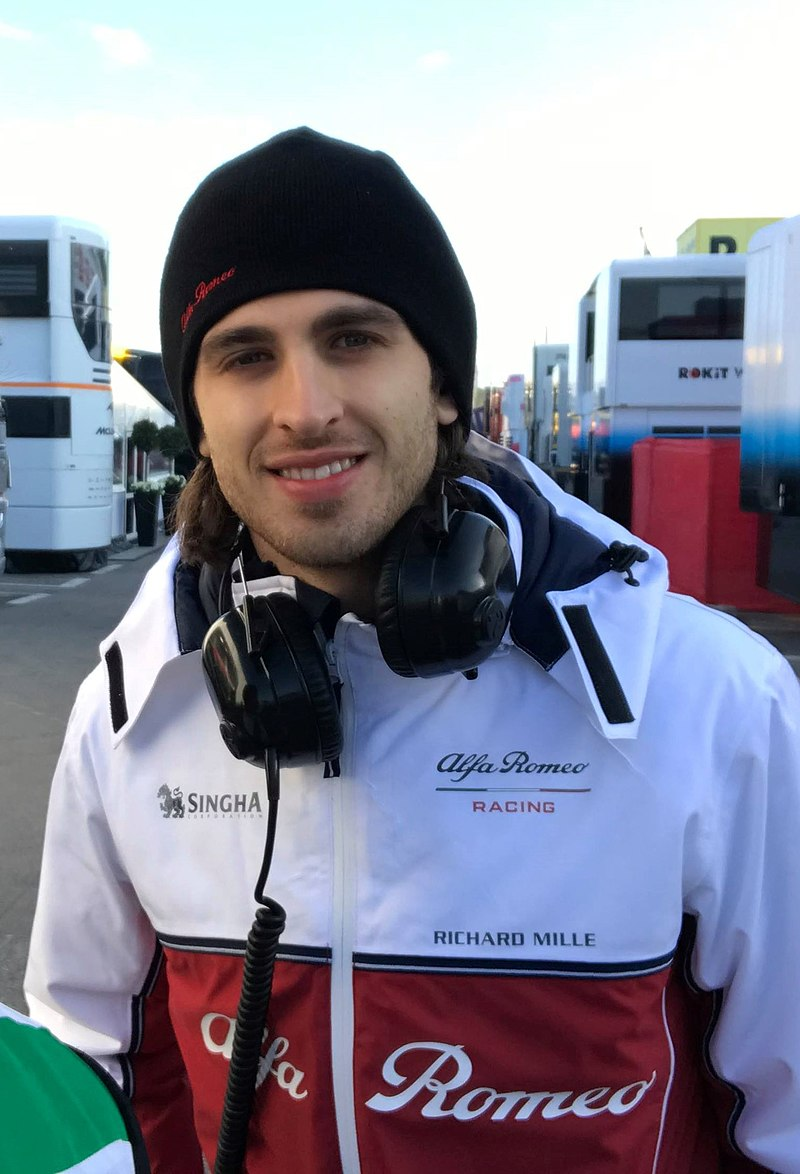
\includegraphics[scale = 0.1]{Fotos/Pilotos/Piloto_AlfaRomeo_Antonio_Giovinazzi.jpg}}{\caption{Antonio Giovinazzi}}
            \end{floatrow}
        \end{figure}
        \end{itemize} \hfill\break
    \item Red Bull Toro Rosso Honda:
        \begin{itemize}
            \item Pierre Gasky
            \item Daniil Kvyat \hfill\break
        \begin{figure}[!h]
            \begin{floatrow}
             \ffigbox{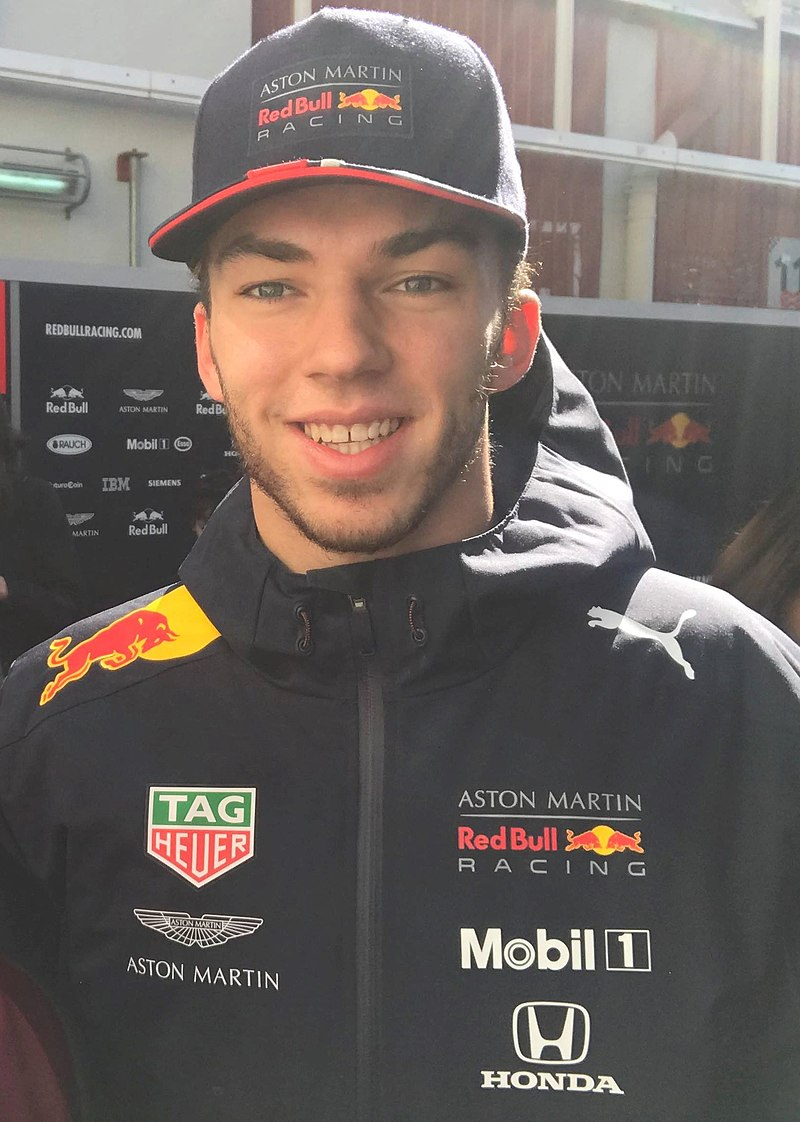
\includegraphics[scale = 0.1]{Fotos/Pilotos/PilotoToroRossoPierreGasly.jpg}}{\caption{Pierre Gasky}}
             \ffigbox{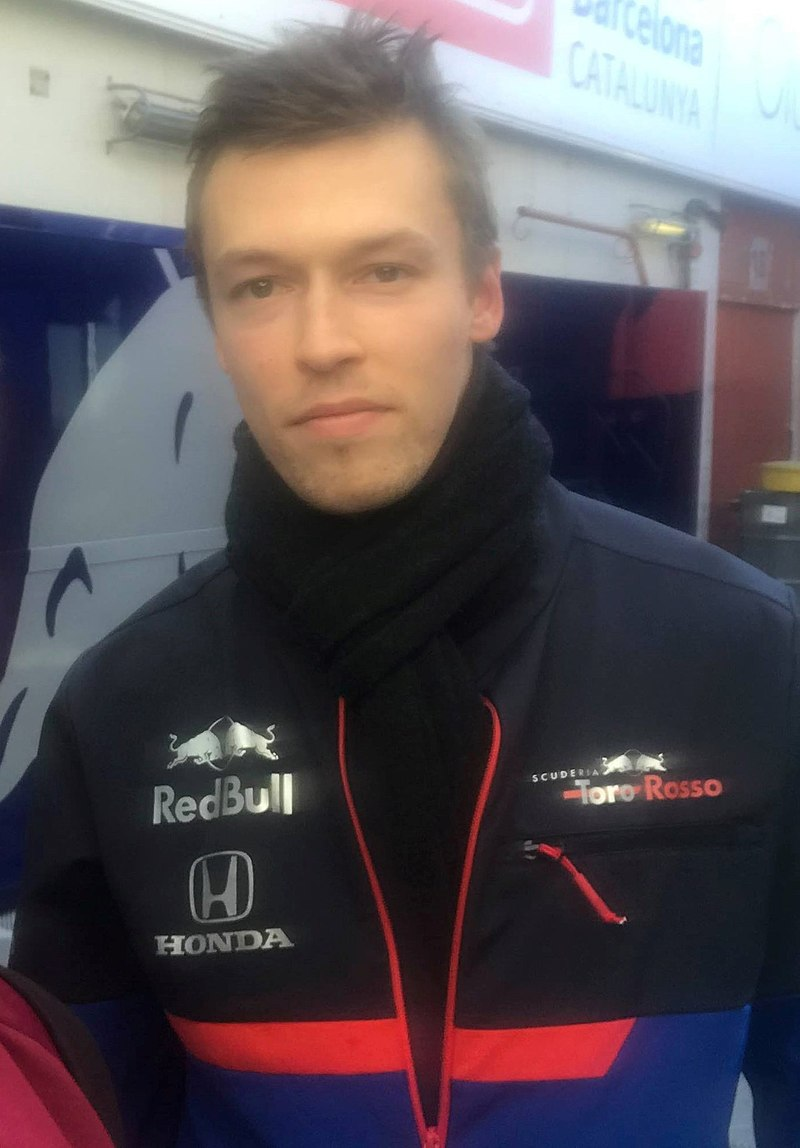
\includegraphics[scale = 0.1]{Fotos/Pilotos/PilotoToroRossoDaniilKvyat.jpg}}{\caption{Daniil Kvyat}}
           \end{floatrow}
        \end{figure}
        \end{itemize} 
    \item Mercedes AMG Pertronas Motorspor:
        \begin{itemize}
            \item Lewis Hamilton
            \item Valteri Bottas \\*
        \begin{figure}[!h]
            \begin{floatrow}
             \ffigbox{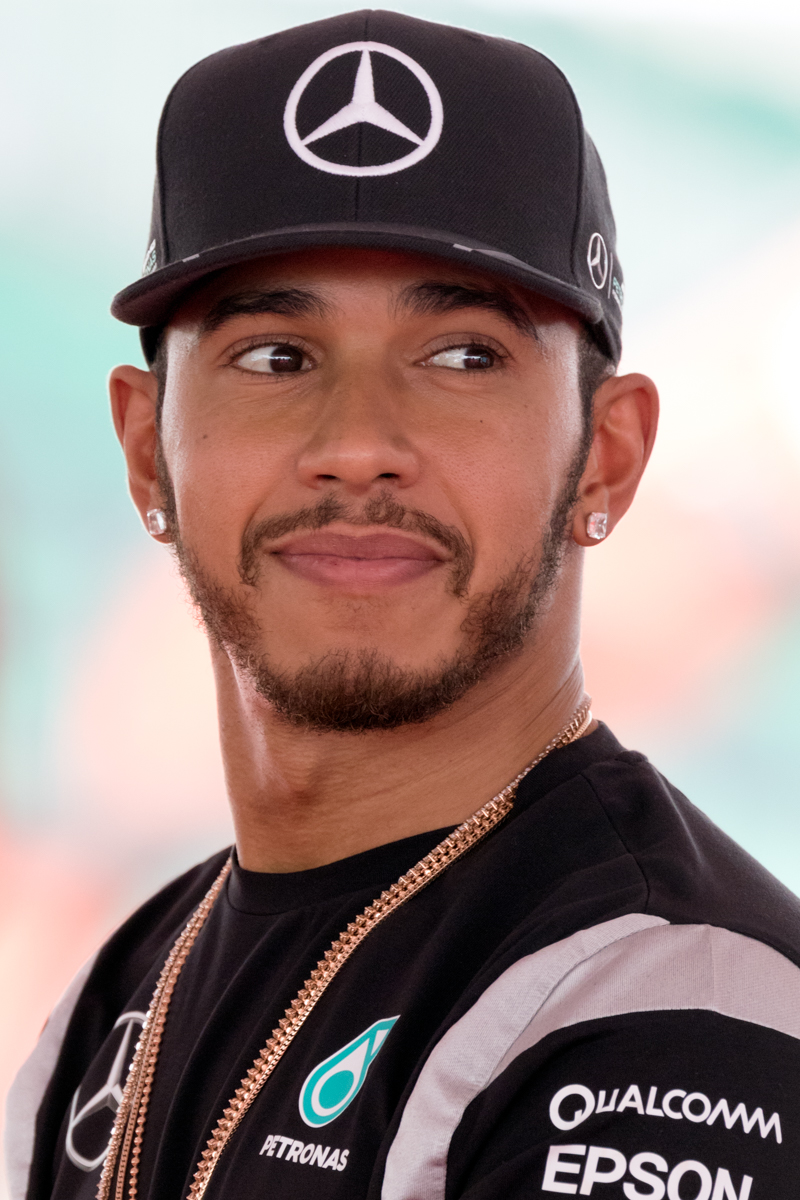
\includegraphics[scale = 0.35]{Fotos/Pilotos/PilotoMercedesLewisHamilton.jpg}}{\caption{Lewis Hamilton}}
             \ffigbox{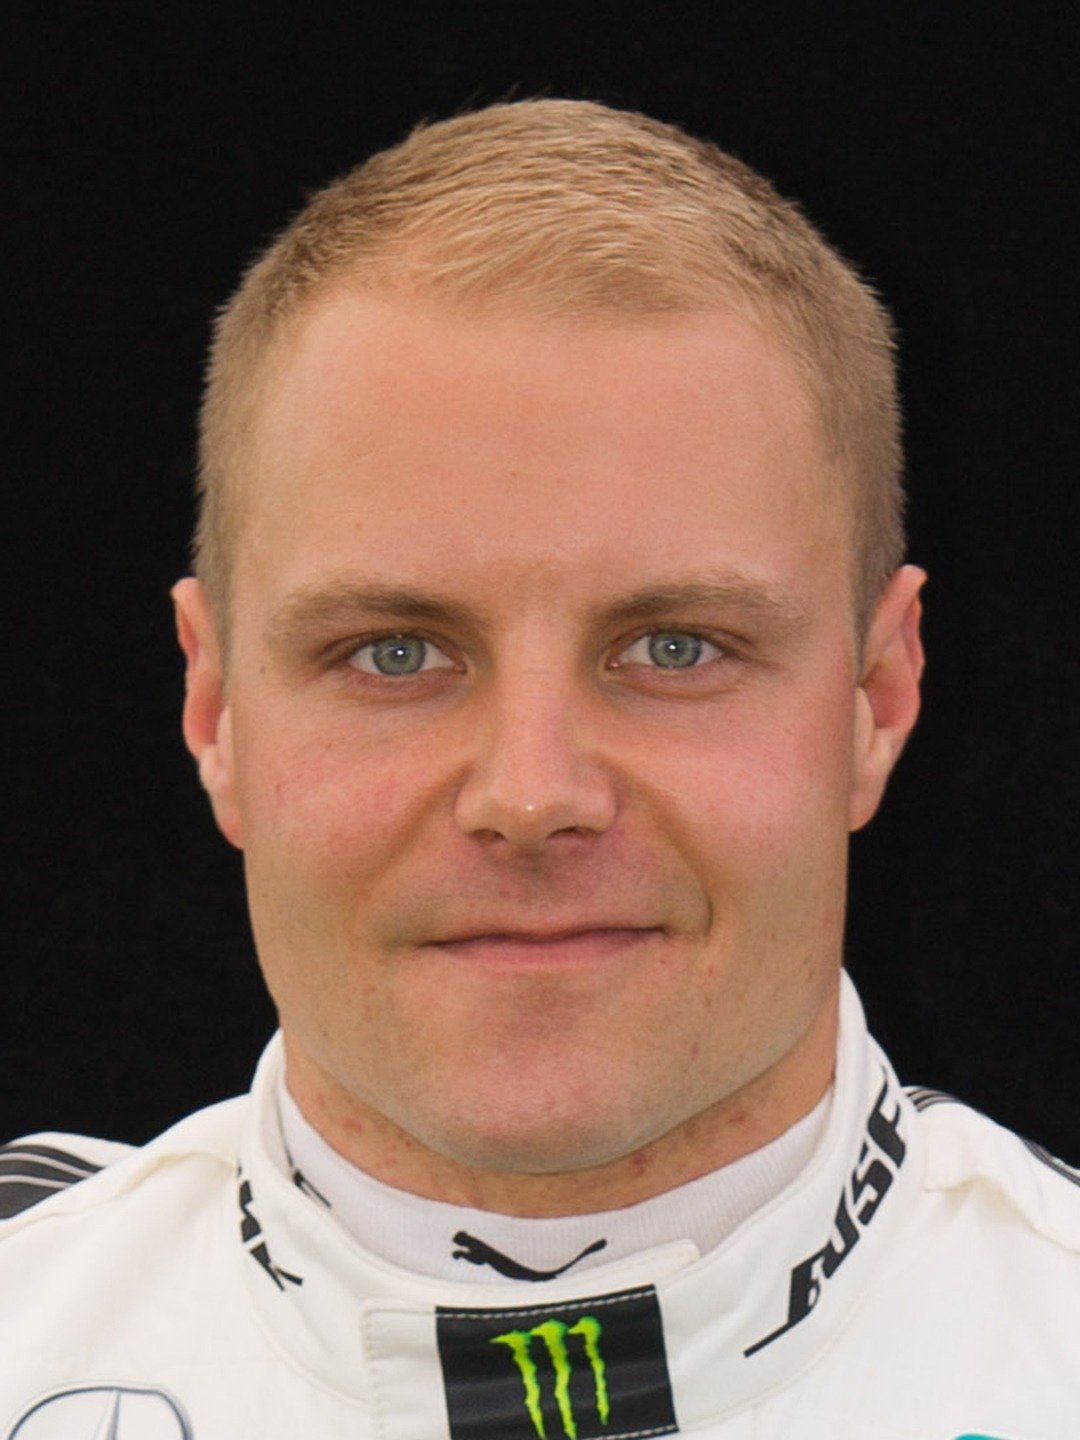
\includegraphics[scale = 0.08]{Fotos/Pilotos/PilotoMercedesValtteriBottas.jpg}}{\caption{Valteri Bottas}}
        \end{floatrow}
        \end{figure}
        \end{itemize}
    \bigskip\bigskip\bigskip\bigskip\bigskip\bigskip\bigskip
    \item ROKit Williams Racing:
        \begin{itemize}
            \item George Russell 
            \item Robert Kubica
            \bigskip
            \begin{figure}[!h]
            \begin{floatrow}
             \ffigbox{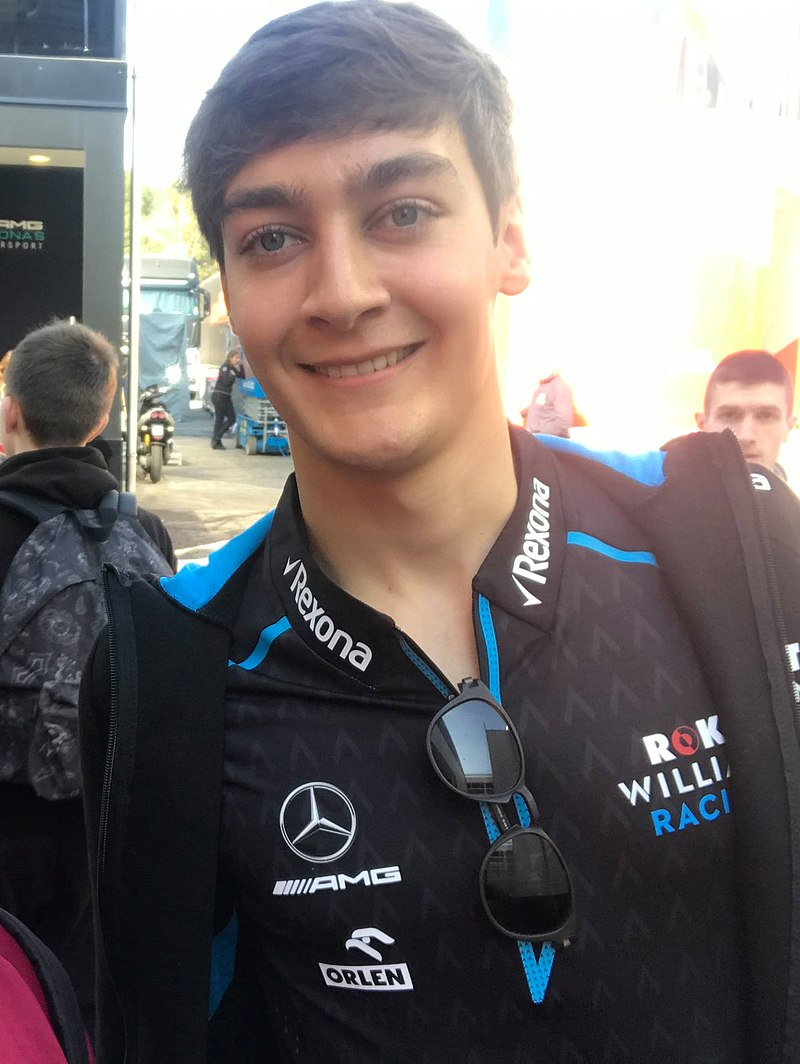
\includegraphics[scale = 0.11]{Fotos/Pilotos/PilotoWilliamsGeorgeRussell.jpg}}{\caption{George Russel}}
             \ffigbox{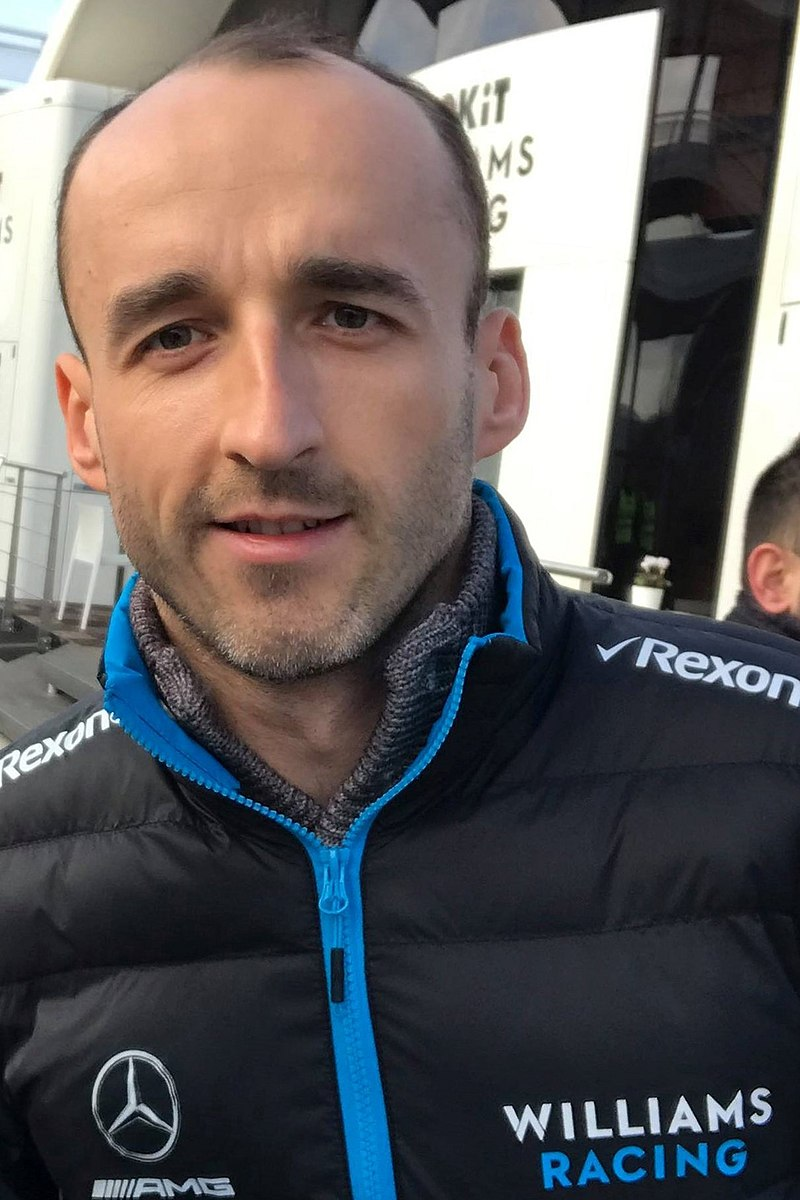
\includegraphics[scale = 0.1]{Fotos/Pilotos/PilotoWilliamsRobertKubica.jpg}}{\caption{Robert Kubica}}
            \end{floatrow}
            \end{figure}
        \end{itemize}
    \item Aston Martin Red Bull Racing: 
        \begin{itemize}
            \item Max Verstappen
            \item Alexander Albon
            \begin{figure}[!h]
            \begin{floatrow}
             \ffigbox{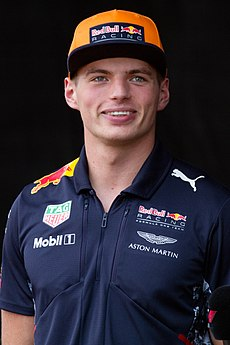
\includegraphics[scale = 0.35]{Fotos/Pilotos/PilotoRedBullMaxVerstappen.jpg}}{\caption{Max Verstappen}}
             \ffigbox{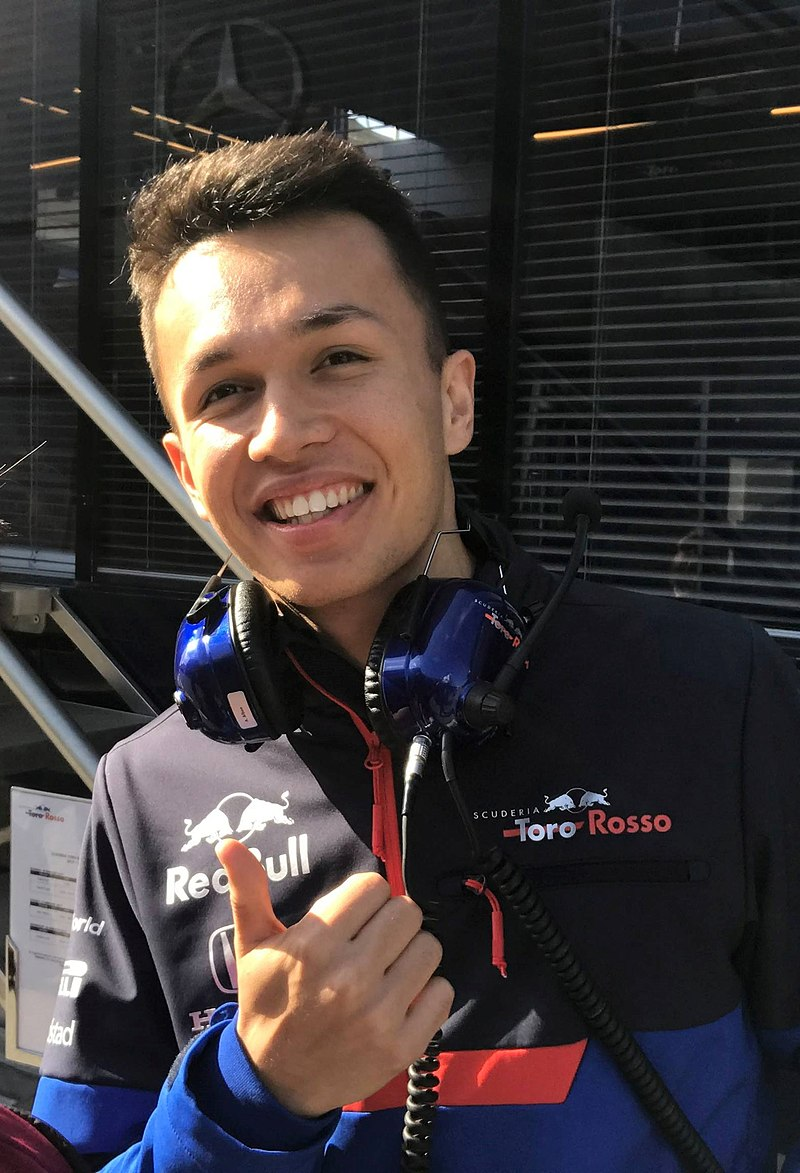
\includegraphics[scale = 0.1]{Fotos/Pilotos/PilotoRedBullAlexenderAlbon.jpg}}{\caption{Alexander Albon}}
            \end{floatrow}
            \end{figure}
        \end{itemize}
    \bigskip\bigskip\bigskip\bigskip\bigskip\bigskip\bigskip\bigskip\bigskip\bigskip\bigskip
    \item Haas F1 Team:
        \begin{itemize}
            \item Romain Grosjean
            \item Kevin Magnussen 
             \begin{figure}[!h]
            \begin{floatrow}
             \ffigbox{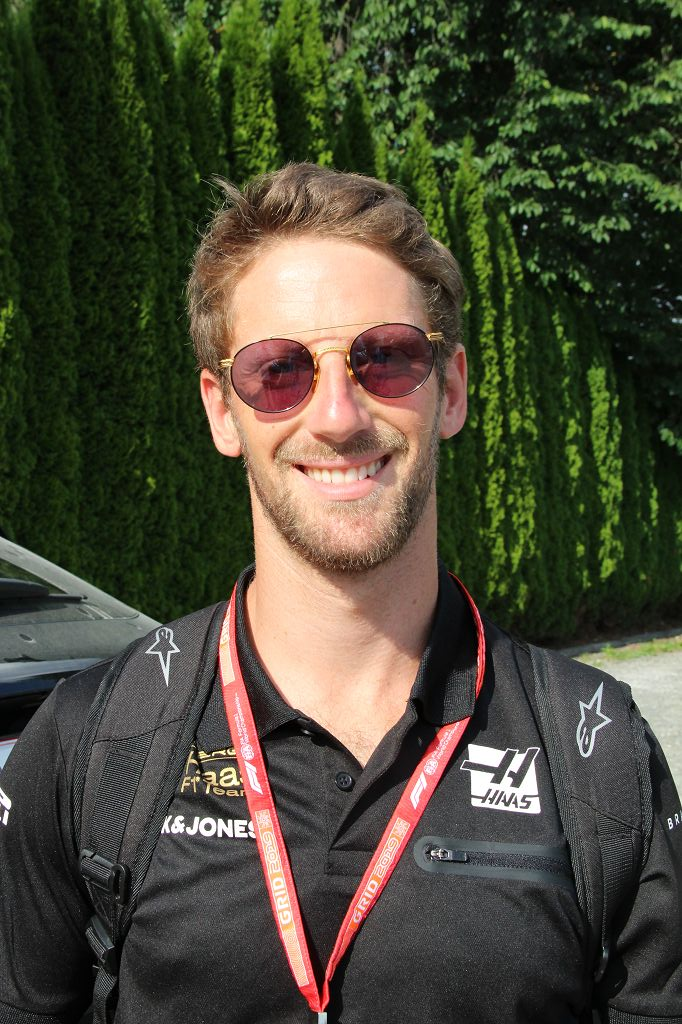
\includegraphics[scale = 0.17]{Fotos/Pilotos/PilotoHaasFerrariRomainGrosjean.jpg}}{\caption{Romain Grosjean}}
             \ffigbox{
\includegraphics[scale = 0.1]{Fotos/Pilotos/PilotoHaasFerrariKevinMagnussen.jpg}}{\caption{Kevin Magnussen}}
            \end{floatrow}
            \end{figure}
        \end{itemize}
    \item McLaren F1 Team:
        \begin{itemize}
            \item Lando Norris 
            \item Carlos Sainsz
             \begin{figure}[!h]
            \begin{floatrow}
             \ffigbox{
\includegraphics[scale = 0.15]{Fotos/Pilotos/PilotoMcLarenLandoNorris.jpg}}{\caption{Lando Norris}}
             \ffigbox{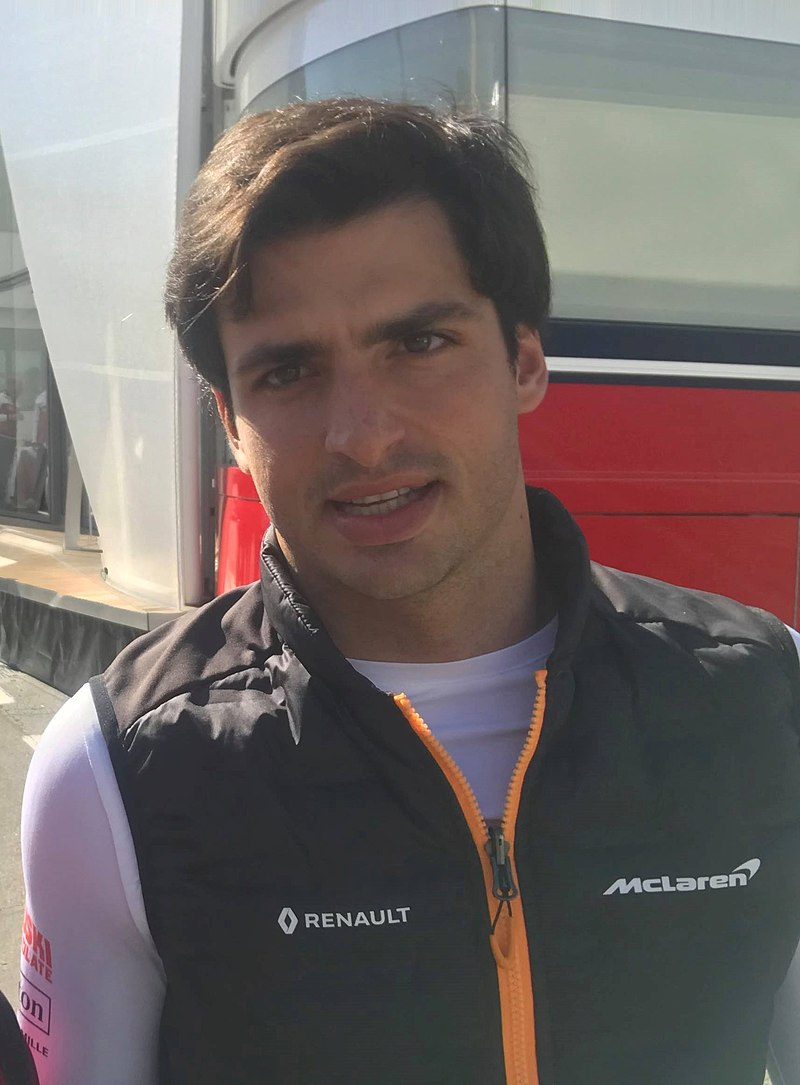
\includegraphics[scale = 0.1]{Fotos/Pilotos/PilotoMcLarenCarlosSainzJr.jpg}}{\caption{Carlos Sainz}}
            \end{floatrow}
            \end{figure}
        \end{itemize}
    \bigskip\bigskip\bigskip\bigskip\bigskip\bigskip\bigskip\bigskip\bigskip\bigskip\bigskip
    \item Scuder Ferrari:
        \begin{itemize}
            \item Chales Leclerc
            \item Sebastian Vettel
            \begin{figure}[!h]
            \begin{floatrow}
             \ffigbox{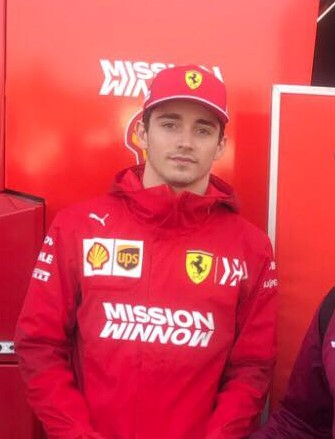
\includegraphics[scale = 0.35]{Fotos/Pilotos/PilotoFerrariChalesLeclerc.jpg}}{\caption{Chales Leclerc}}
             \ffigbox{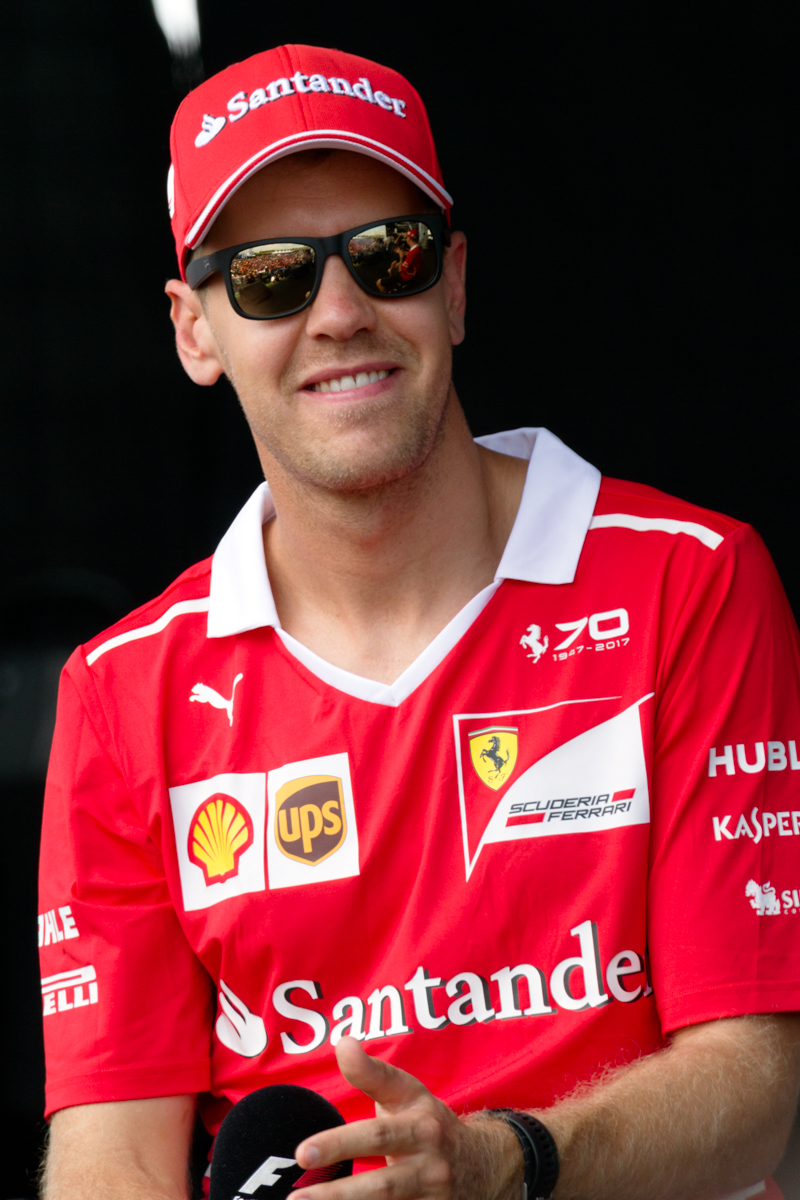
\includegraphics[scale = 0.31]{Fotos/Pilotos/PilotoFerrariSebastianVettel.jpg}}{\caption{Sebastian Vettel}}
            \end{floatrow}
            \end{figure}
        \end{itemize}
    \item Sport Pesa Racing Point F1 Team :
        \begin{itemize}
            \item Sergio Pérez
            \item Lance Stroll
            \begin{figure}[!h]
            \begin{floatrow}
             \ffigbox{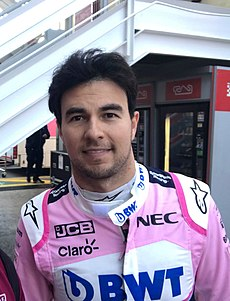
\includegraphics[scale = 0.4]{Fotos/Pilotos/PilotoRacingPointSergioPerez.jpg}}{\caption{Sergio Pérez}}
             \ffigbox{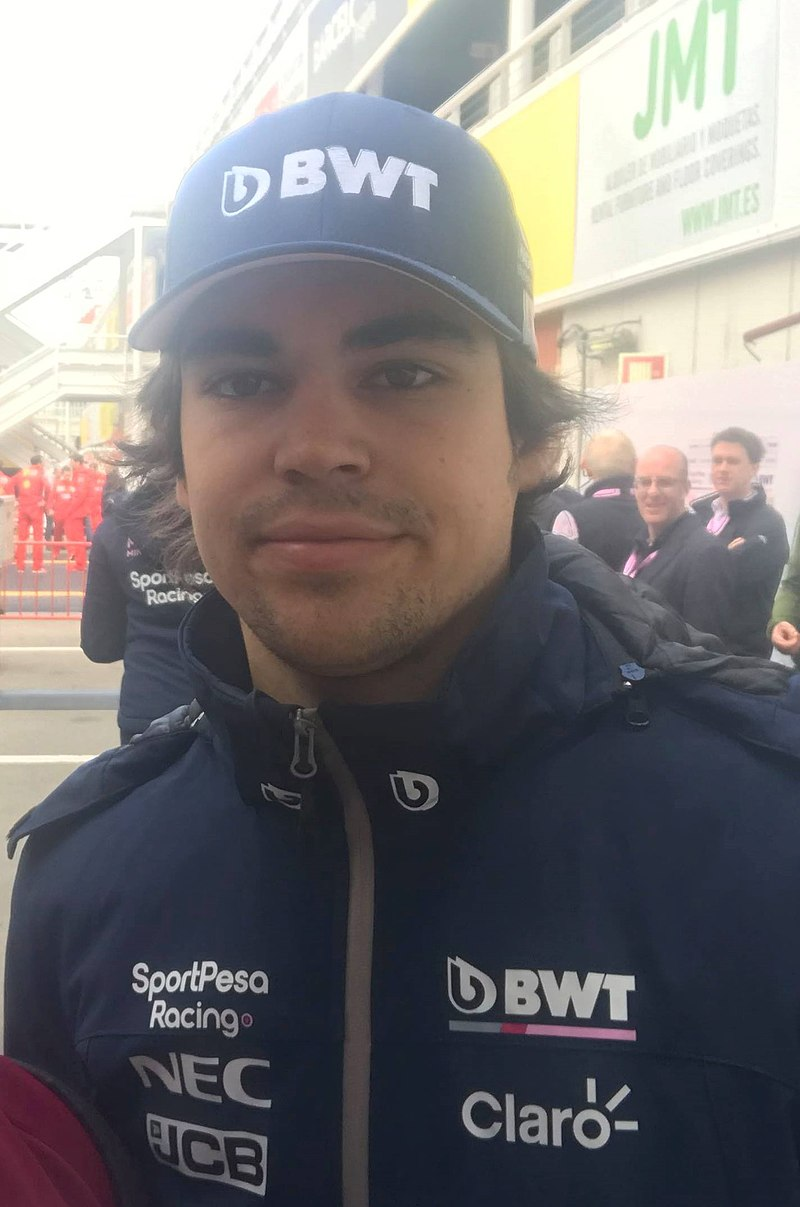
\includegraphics[scale = 0.1]{Fotos/Pilotos/PilotoRacingPointLanceStroll.jpg}}{\caption{Lance Stroll}}
            \end{floatrow}
            \end{figure}
        \end{itemize}
    \bigskip\bigskip\bigskip\bigskip\bigskip\bigskip\bigskip\bigskip\bigskip\bigskip\bigskip\bigskip\bigskip\bigskip
    \item Renault F1 Team:
        \begin{itemize}
            \item Daniel Ricciardo
            \item Nico Hulkenberg
            \begin{figure}[!h]
            \begin{floatrow}
             \ffigbox{
\includegraphics[scale = 0.12]{Fotos/Pilotos/PilotoRenaultDanielRiccciardo.jpg}}{\caption{Daniel Ricciardo}}
             \ffigbox{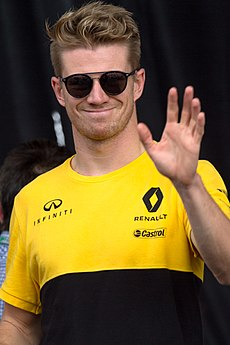
\includegraphics[scale = 0.35]{Fotos/Pilotos/PilotoRenaultNicoHulkenberg.jpg}}{\caption{Nico Hulkenberg}}
            \end{floatrow}
            \end{figure}
        \end{itemize}
    
    
\end{itemize}
\section{Calendário da \ac{f1}}
Atualmente, o calendário da \ac{f1} conta com 19 provas, acontecendo estas de 2 em 2 semanas salvo algumas exceções.
Assim sendo, a temporada começa com o icónico \textbf{\ac{gp} de Melbourne, Austrália}, em Fevereiro em que as equipas vão testar pela primeira vez os seus carros. De seguida temos os \textbf{\ac{gp}de Sakhir, Bahrain}, o \textbf{\ac{gp} de Shangai na China}, o de \textbf{Baku no Azerbeijão}, o \textbf{\ac{gp} de Barcelona em Espanha}. Depois temos o \textbf{\ac{gp} de Monte Carlo, no Mónaco}, que é o único \ac{gp} que tem o seu dia de treinos na quinta-feira, pois a sexta-feira está reservada para eventos de marketing. Segues-se o \textbf{\ac{gp} de Montreal, Canadá}, o de \textbf{Paul Ricard em França}, o \textbf{\ac{gp} de Spielberg na Áustria}, o icónico \textbf{\ac{gp} de Silverstone, em Inglaterra}, o de \textbf{Hockenheim na Alemanha}, e o de \textbf{Hungaroring na Hungria}. Depois é a pausa de verão que dura três semanas, e a ação retorna com o longo \textbf{\ac{gp} de Spa-Francorchamps na Bélgica}, seguido pelo vibrante \textbf{\ac{gp} de Monza em Itália}, o de \textbf{Sochi, na Rússia} e o de \textbf{Suzuka, no Japão}. Depois a competição salta para o continente americano, onde decorrerá o \textbf{\ac{gp} de Hermanos Rodríguez no México}, seguido pelo \textbf{\ac{gp} de Austin, nos Estados Unidos da América} e acabando esta \textit{tour} americana no \textbf{\ac{gp} de Interlagos no Brasil}. A temporada acaba no \textbf{\ac{gp} de Yas Marina, em Abu Dhabi}, no fim de Novembro.  
\section{Merchandising}
Atualmente, a \ac{f1} é muito mais ativa nas redes sociais e noutras plataformas de comunicação do que era antigamente. Assim sendo é muito comum encontrarmos anúncios de \ac{gp} no Twitter, Facebook. No Youtube a \ac{f1} conta com um canal com mais de 3 milhões de subscritores, onde são postados os melhores momentos de cada corrida, assim como momentos marcantes da história da competição.

Recentemente, a série lançada pela \textit{Netflix}, Drive to Survive, foi um sucesso e atraiu muitos jovens a ver este desporto. Foi confirmado uma segunda temporada da mesma série. 

Outra situação que ajuda a promover a categoria é todo o vestuário associados às equipas. Assim sendo, é muito comum ver fãs a envergar as camisolas das suas equipas preferidas, que podem ser obtidas pela loja online da \ac{f1}, ou pelas lojas das equipas.
\\
\newline
Links das redes sociais da \ac{f1}:
\begin{itemize}
    \item Youtube: \url{https://www.youtube.com/user/Formula1}
    \item Twitter: \url{https://twitter.com/F1}
    \item Facebook: \url{https://www.facebook.com/Formula1/}
    \item Site: \url{https://formula1.com}
    \item Loja Online: \url{https://f1store.formula1.com/stores/f1/en/c/}
\end{itemize}

\chapter{Regras}
\label{chap.regras}
\hspace{\parindent}Atualmente, o regulamento da \ac{f1} é estabelecido pela \ac{fia}, última vez editado em 12 de março de 2019\footnote[1]{https://www.fia.com/regulation/category/110 (consultado a 26 de novembro de 2019)}. É de notar que as regras aqui presentes estão de acordo com o regulamento atual e que este regulamento é alterado periodicamente, de modo a manter a integridade e competitividade do desporto.

Existem vários tipos de regras como por exemplo: \cite{wikipedia}
\begin{itemize}
   \item É obrigatório que todas as equipas sejam formadas por dois pilotos;
   \item É obrigatório que todas as equipas possuam dois carros e que se conformem dentro das regras técnicas aplicadas
   aos mesmos;
   \item Em cada Grande Prémio, todos os pilotos podem participar em duas sessões de treino livre de 1 hora e meia nas sextas-feiras.
   \item O nome ou logótipo da equipa deve aparecer na frente do carro. O nome do piloto também deve de estar presente no chassis do carro.
   \item Todos os carros devem mostrar o número do piloto. Os números dos pilotos são permanentes e serão utilizados em toda a sua carreira na \ac{f1}, em exeção do atual campeão Lewis Hamilton, a quem foi dado a opção de usar o número "1".
 \end{itemize}
\section{Sistema de Pontuações}
\hspace{\parindent}No campeonato existem duas competições externas ao Grande Prémio, o campeonato mundial de pilotos e o campeonato mundial de construtores. O campeonato de pilotos visa premiar o piloto que acumulou mais pontos na \ac{f1}, enquanto que o campeonato de construtor visa premiar a equipa que acumulou mais pontos na \ac{f1}, a pontuação desta equipa é igual à soma das pontuações dos seus pilotos. A única maneira de receber pontos é participando no Grande Prémio e obter uma classificação igual ou superior à 10ª posição.

Os pontos são distribuídos pela seguinte classificação:
\begin{enumerate}
    \item 25 pontos;
    \item 18 pontos;
    \item 15 pontos;
    \item 12 pontos;
    \item 10 pontos;
    \item 8 pontos;
    \item 6 pontos;
    \item 4 pontos;
    \item 2 pontos;
    \item 1 ponto;
\end{enumerate}

A única vez que esta tabela não é aplicada é quando uma prova é suspensa e não puder ser retomada, neste caso se o Grande Prémio tiver menos de 75\% da sua distância percorrida, apenas serão contabilizados metade dos pontos, se menos de duas voltas foram completadas, nenhum ponto será atribuído aos pilotos.
\section{Penalizações}

Os pilotos e/ou as equipas podem ser penalizados pela \ac{fia} quando estes demonstram conduta imprópria e antidesportiva, que prejudique a integridade do desporto e/ou ponha em risco a segurança dos envolvidos. Estas decisões são tomadas pela \ac{fia} durante o decorrer da prova e são acompanhadas pela sinalização da bandeira Metade Preta, Metade Branca na Diagonal ver \ref{Bandeiras}.

O sistema de penalizações da FIA se divide em 6 tipos:
\begin{itemize}
    \item \textbf{Cinco segundos de Penalização de Tempo:} O piloto deve parar no \textit{pit lane} (zona da pista onde se encontram as garagens das equipas) na sua posição \textit{pit stop} (zona encostada à sua \textit{box}, utilizada para reparações de veículo e troca de pneus) pelo menos durante 5 segundos, em seguida, pode realizar a troca de pneus ou reparações no carro, se assim o desejar. Caso o piloto não opte por ir à \textit{pit lane}, está proibido de aceder a essa zona até ao fim da corrida e irão ser adicionados 5 segundos ao seu tempo de corrida.
    \item \textbf{Dez segundos de Penalização de Tempo:} O piloto deve parar no \textit{pit lane} na sua posicão \textit{pit stop} pelo menos durante 10 segundos, em seguida, pode realizar a troca de pneus ou reparações no carro, se assim o desejar. Caso o piloto não opte por ir à \textit{pit lane}, está proibido de aceder a essa zona até ao fim da corrida e irão ser adicionados 10 segundos ao seu tempo de corrida.
    \item \textbf{\textit{Drive-trough:}} Aplicada em pequenas infrações, o piloto terá que aceder à \textit{pit lane}, mas não tem que fazer paragem obrigatória na \textit{pit stop}.
    \item \textbf{\textit{Stop and Go:}} O piloto deverá aceder à \textit{pit lane} e parar durante 10 segundos na sua \textit{pit stop}, no entanto, não são permitidas reparações no carro.
    \item \textbf{Perda de Posições:} Resulta de infrações graves, como: ultrapassagem ilegal e condução perigosa. Nesses casos são adicionadas 10 posições à posição atual do piloto.
    \item \textbf{Suspensão:} O piloto e/ou a equipa que cometeram infrações graves, como por exemplo batota, serão suspensos da temporada atual, após decisão judicial.
\end{itemize}
\section{Bandeiras}

As bandeiras são um ícone dos desportos motorizados, na \ac{f1} as bandeiras desempenham a função crucial de transmitir informação rápida aos pilotos que estão a correr. Os avisos podem ser transmitidos via rádio, mas como estes podem ter não funcionar durante o Grande Prémio e normalmente estes avisos são críticos, opta-se por usar este sistema de bandeiras. Atualmente, as bandeiras da \ac{f1} são produzidas por uma empresa Americana chamada \textit{Pantone}, mas ao contrário dos pneus utilizados na \ac{f1}, o código de cores é responsabilidade da \ac{fia}.
\begin{table}[!h]
\large
\centering
\resizebox{\textwidth}{!}{
\begin{tabular}{|c|l|l|c|c|l|l|l|l|l|l|l|}
\hline
\multicolumn{3}{|c|}{Bandeira} & Cor                                                                                   & \multicolumn{8}{c|}{Significado}  \\ \hline
\multicolumn{3}{|c|}{
\includegraphics[]{Fotos/Bandeira/Bandeira_Amarela.png}}         & Amarela                                                                               & \multicolumn{8}{c|}{\begin{tabular}[c]{@{}c@{}}\textbf{1 Bandeira:} Perigo adiante, detritos resultantes de acidente. \\ Os pilotos devem reduzir a velocidade ao cruzar o local do acidente.\\ \textbf{2 Bandeiras:} Muito perigo adiante. Os pilotos devem \\ preparar-se para uma eventual parada.\\ \textbf{1 Bandeira e Placa de VSC:}\footnote[1]{\ac{vsc} placa virtual que imita a presença de um \ac{sc}.} Os pilotos terão de respeitar uma \\ velocidade imposta pela FIA. Quem não respeitar, poderá ser penalizado.\\ \textbf{1 Bandeira e Placa SC:} Entrada do \textit{safety car}. \\ Os pilotos devem reduzir a velocidade\end{tabular}} \\ \hline
\multicolumn{3}{|c|}{
\includegraphics[]{Fotos/Bandeira/Bandeira_Verde.png}}         & Verde                                                                                 & \multicolumn{8}{c|}{A pista está liberada e os pilotos podem retomar suas posições.} \\ \hline
\multicolumn{3}{|c|}{
\includegraphics[]{Fotos/Bandeira/Bandeira_Vermelha.png}}         & Vermelha                                                                              & \multicolumn{8}{c|}{\begin{tabular}[c]{@{}c@{}}A prova foi suspensa. Os carros que estiverem a percorrer o \\ circuito devem reduzir e seguir até linha vermelha.\end{tabular}} \\ \hline
\multicolumn{3}{|c|}{
\includegraphics[]{Fotos/Bandeira/Bandeira_Azul.png}}         & Azul                                                                                  & \multicolumn{8}{c|}{\begin{tabular}[c]{@{}c@{}}O carro mais lento deve dar passagem a um carro mais veloz que quer ultrapassar. \\ O piloto que ignorar até três bandeiradas leva a penalização\\ (Drive-trough ou Stop and Go).\end{tabular}} \\ \hline
\multicolumn{3}{|c|}{
\includegraphics[]{Fotos/Bandeira/Bandeira_Branca.png}}         & Branca                                                                                & \multicolumn{8}{c|}{Entrada de carro lento na pista. Pilotos devem reduzir a velocidade.} \\ \hline
\multicolumn{3}{|c|}{
\includegraphics[]{Fotos/Bandeira/Bandeira_Preta.png}}         & Preta                                                                                 & \multicolumn{8}{c|}{\begin{tabular}[c]{@{}c@{}}Desclassificação. O piloto que a recebeu deve retornar à box.\\ Vem acompanhada com o número do piloto.\end{tabular}} \\ \hline
\multicolumn{3}{|c|}{
\includegraphics[]{Fotos/Bandeira/Bandeira_Xadrez.png}}         & Xadrez                                                                                & \multicolumn{8}{c|}{\begin{tabular}[c]{@{}c@{}}Fim da etapa. Indica a vitória do primeiro a cruzar a linha.\\\end{tabular}} \\ \hline
\multicolumn{3}{|c|}{
\includegraphics[]{Fotos/Bandeira/Bandeira_PB.png}}         & \begin{tabular}[c]{@{}c@{}}Metade Preta,\\Metade Branca\\na Diagonal\end{tabular} & \multicolumn{8}{c|}{\begin{tabular}[c]{@{}c@{}}Indica que o piloto desempenhou atitude antidesportiva, à qual fica sob\\ a ameaça de desclassificação. \\ Vem acompanhada do número do piloto.\end{tabular}} \\ \hline
\multicolumn{3}{|c|}{
\includegraphics[]{Fotos/Bandeira/Bandeira_LP.png}}         & \begin{tabular}[c]{@{}c@{}}Preta com\\Círculo\\Laranja\end{tabular}                   & \multicolumn{8}{c|}{\begin{tabular}[c]{@{}c@{}}Indica que há um problema técnico com o carro. O piloto em questão (indicado\\ na bandeira) deve ir à box.\end{tabular}} \\ \hline
\multicolumn{3}{|c|}{
\includegraphics[]{Fotos/Bandeira/Bandeira_VA.png}}         & \begin{tabular}[c]{@{}c@{}}Listrada em\\Amarelo\\e preto\end{tabular}                 & \multicolumn{8}{c|}{\begin{tabular}[c]{@{}c@{}}Indica a presença de detritos ou óleo na pista.\\ Os pilotos devem de reduzir a  velocidade a partir do ponto sinalizado.\end{tabular}} \\ \hline
\end{tabular}
}
\caption{Código de cores das Bandeiras}
\label{Bandeiras}
\end{table}
\section{Pneus}
\hspace{\parindent}Atualmente, todos os pneus utilizados na \ac{f1} são fornecidos pela marca italiana \textit{Pirelli}. Cada equipa recebe 20 conjuntos de pneus para cada Grande Prémio, sendo destes 13 conjuntos para pista seca, 4 conjuntos para pista mista e 3 conjuntos para pista molhada.

Tanto para pista mista, como para a pista molhada só existe um tipo de composto para o pneu, para pista mista: Intermediário e para pista molhada: Chuva. Para pista são disponibilizados 3 tipos de compostos para pneus: Macio, Médio, Duro ver \ref{Tipos de Pneus}. O número de conjuntos de cada composto é escolhido por cada equipa. \textbf{Nota:} Todas as equipas devem de usar (no mínimo) dois tipos de pneus para pistas secas durante a corrida.
\begin{table}[!h]
\centering
\begin{tabular}{|c|l|l|c|c|}
\hline
\multicolumn{3}{|c|}{Composto} & \multicolumn{2}{c|}{Cor} \\ \hline
\multicolumn{3}{|c|}{Macio}    & \cellcolor[HTML]{FD6864}{\color[HTML]{000000} Vermelho} & 
\includegraphics[scale=0.33]{Fotos/Pneus/Pneu_Vermelho.png} \\ \hline
\multicolumn{3}{|c|}{Médio}    & \cellcolor[HTML]{FCFF2F}Amarelo                         &  
\includegraphics[scale=0.017]{Fotos/Pneus/Pneu_Amarelo.png} \\ \hline
\multicolumn{3}{|c|}{Duro}     & \cellcolor[HTML]{FFFFFF}Branco                          &  
\includegraphics[scale=0.017]{Fotos/Pneus/Pneu_Branco.png} \\ \hline
\end{tabular}
\caption{Tipos de Pneus}
\label{Tipos de Pneus}
\end{table}
\chapter{Impacto da Fórmula 1 no nosso quotidiano}
\label{chap.impactof1}
\hspace{\parindent}Durante décadas, a \ac{f1} não foi só a rainha dos desportos motorizados, foi também o laboratório de pesquisa e desenvolvimento mais rápido do mundo, as inovações feitas nesta modalidade foram, inevitavelmente, desencadear inovação e melhorias na tecnologia utilizada pelos carros do nosso quotidiano.

Foi a industria da \ac{f1} que começou a desenvolver os sensores de telemetria mais avançados que hoje podem ser encontrados em carros comerciais, aumentando a conectividade entre o condutor e o veiculo, dentro desta categoria encontramos funções como: alerta da pressão dos pneus, altera de proximidade de objetos, reconhecimento da via, entre outros. Devido à necessidade de motores mais fortes, leves e compactos, a \ac{f1} é responsável pelo desenvolvimento da tecnologia que aumentou a eficiência térmica nunca antes alcançada, os carros comerciais a \textit{diesel} já começam a tirar proveito deste novo avanço tecnológico.

Vistos que estes carros estão repletos de sensores que, vão ser analisados nas \textit{boxes} das equipas, estas precisam de ter um centro de dado equivalentes a uma pequena empresa. Devido ao ambiente hostil que contem: altas vibrações, uma grande quantidade de fumos e, por vezes, temperaturas extremas. Estas equipas tiveram que desenvolver tecnologias que permitissem o uso de uma base de dados nesses locais.

Esta modalidade também é responsável pelo progressos no domínio da Engenharia de Materiais, devido à necessidade de materiais mais leves e resistentes.
\chapter{Curiosidades}
\label{chap.curiosidades}
\hspace{\parindent}Como pode ser visto, a \ac{f1} é um desporto muitíssimo versátil, capaz de alcançar os pontos de interesse de muitos indivíduos, devido à sua ampla área de trabalho. É normal que um desporto como este tenha por de trás factos que até possam surpreender os mais conhecedores desta modalidade. Dentro desta categoria temos algumas curiosidades, como:
\begin{itemize}
    \item A morte de Ayrton Senna fez com que a segurança avançasse imenso na prova.
    \item Michael Schumacher é o piloto mais condecorado de sempre, com 7 campeonatos mundiais. Lewis Hamilton está na "caça" deste feito contando já com 6 campeonatos.
    \item Max Verstappen é o piloto  mais novo de sempre a ter guiado um carro de \ac{f1}, tendo-o feito com 17 anos e 2 dias. A partir daí tornou-se ilegal ter pilotos a competir com menos de 18 anos de idade.
    \item A Ferrari é a equipa com mais títulos, tendo 16 Campeonatos de Construtores e 15 Campeonatos de Pilotos, sendo seguida pela McLaren.
    \item Um carro da \ac{f1} consegue ir dos 0 \ac{kmh} até 160 \ac{kmh}, de volta aos 0 \ac{kmh} em 4 segundos.
    \item O preço base de um carro utilizado na \ac{f1} ronda o 7 milhões de dólares.
    \item As equipas participantes na \ac{f1} conseguem mudar os pneus do seu carro em 3 segundos.
    \item O motor de um carro \ac{f1} dura menos de 5 corridas.
    \item Um piloto perde à volta de 4 \ac{kg} durante uma corrida.
    \item Cada pneu costuma perder 0,5 \ac{kg} durante uma utilização em corrida.
    \item Só uma mulher é que conseguiu pontoar no Grande Prémio e o seu nome era Lella Lombardi.
    \item Os discos dos travões podem atingir até 1000 \ac{gc}.
    \item O motor dos carros da \ac{f1} não conseguem funcionar frios, normalmente são pré-aquecidos antes de serem usados.
\end{itemize}
\chapter{Conclusões}
\label{chap.conclusoes}
\hspace{\parindent}A partir da informação apresentada concluímos que este desporto motorizado é bastante amplo e assim, consegue atingir os interesses pessoais de qualquer pessoa, já que pisa nos domínios do Marteking, da Tecnologia da Comunicação, da Engenharia dos Materiais, do Design, da Aerodinâmica, da Engenharia Física e muitos mais. Apesar de ser uma modalidade simples para o espectador casual, demonstra uma grande complexidade no seu interior que consegue captar o interesse dos espectadores mais interessados pela \ac{f1}.

É notório que este desporto contribuiu, de certa forma, para a maneira de como hoje vivemos, sem ele a nossa vida podia ser radicalmente diferente no que toca às nossa condução e as novas tecnologias das telecomunicações.

Este trabalho também serviu para aprofundar o conhecimento dos autores sobre este assunto, devido às horas gastas a filtrar informação e conhecer mais sobre este maravilhoso mundo da \ac{f1}.
\chapter*{Contribuições dos autores}
\hspace{\parindent}O tema deste trabalho foi escolhido por ambos os autores e houve uma distribuição equitativa de tarefas. O resumo e os agradecimentos e a introdução do trabalho foram também realizados em conjunto, dividindo o resto do capítulos igualmente pelos autos. O \textbf{JS} realizou a Introdução, a História da Fórmula 1 e a Fórmula 1 Atual, enquanto que o \textbf{AC} realizou as Regras, o Impacto da Fórmula 1 no nosso quotidiano, as Curiosidades e as Conclusões. Cada uma contribuiu 50\% para este trabalho.
%%%%%%%%%%%%%%%%%%%%%%%%%%%%%%%%%
\chapter*{Acrónimos}
\begin{acronym}
\acro{bhp}[bhp]{brake horsepower}
\acro{cc}[cc]{Centímetros Cúbicos}
\acro{f1}[F1]{Fórmula 1}
\acro{fia}[FIA]{\textit{Fédération Internationale de l'Automobile}}
\acro{fisa}[FISA]{\textit{Federacion Internationale du Sport Automobile}}
\acro{foca}[FOCA]{\textit{Formula One Constructors Association}}
\acro{gc}[ºC]{Graus Celsius}
\acro{gp}[GP]{Grande Prémio}
\acro{kg}[Kg]{Quilogramas}
\acro{kmh}[Km/h]{Quilómetros por hora}
\acro{labi}[LABI]{Laboratórios de Informática}
\acro{miect}[MIECT]{Mestrado Integrado em Engenharia de Computadores e Telemática}
\acro{sc}[SC]{\textit{Safety Car}}
\acro{vsc}[VSC]{\textit{Virtual Safety Car}}
\acro{ua}[UA]{Universidade de Aveiro}
\end{acronym}
%%%%%%%%%%%%%%%%%%%%%%%%%%%%%%%%%
\printbibliography
\end{document}